\documentclass[sansserif, 10pt]{beamer}
\usepackage{graphicx}
\usepackage{subcaption}
\usepackage{amsfonts}
\usepackage{amsmath}
\usepackage{algorithm2e}
\usepackage{rotating}
\usepackage{/home/sci/weiliu/haldefs}
\usepackage{media9}
\usepackage{tikz}
\usepackage{calligra}

\usetheme{Warsaw}
\useinnertheme{rectangles}

\setbeamertemplate{headline}{} % remove section from header.
\setbeamertemplate{navigation symbols}{}
\renewcommand\mathfamilydefault{\rmdefault}
\renewcommand{\inserttotalframenumber}{52}
\setbeamertemplate{footline}[page number] % add page number
\setbeamerfont{institute}{size=\large}
\setbeamerfont{author}{size=\large}


\title[Resting-State Functional MRI Analysis by Graphical Model]{Resting-State
  Functional MRI Analysis by~Graphical Model}

\subtitle{With Applications on Functional Network Estimation}
\author[W. Liu]{Wei Liu}
\institute[SCI]{
  Scientific Computing and Imaging Institute\\
  University of Utah\\
  Advisor: Tom Fletcher\\
  Co-advisor: Suyash Awate
}
\date{November 25, 2013}
\titlegraphic{
\includegraphics[height=1cm]{sfig/SCI_logo_mono} \hspace{2cm}
\includegraphics[height=1cm]{sfig/ulogo}}
\begin{document}

% 1) fMRI measures the blood oxygenation, and indirectly detect the neuronal
% activity. 2) fMRI have been widely used for the neural basis of the
% perception, cognition and emotion. 3) traditionally has been focusing on the
% regions that shows task-related increases in neural activity. 4) rs-fMRI
% detects the neuronal activity during rest.

% Why interested in resting-state? 1) some regions has greater activity in
% baseline state than during experimental task (DMN) 2) enhance understanding of
% neural activity in baseline states. 3) refine interpretation of activation and
% deactivation.

% mental process. 

% The DMN is only slightly disrupted during passive sensory processing task, but
% is suspended during cognitively demanding external tasks. 

\begin{frame}
  \frametitle{Extended GrabCut Model}
  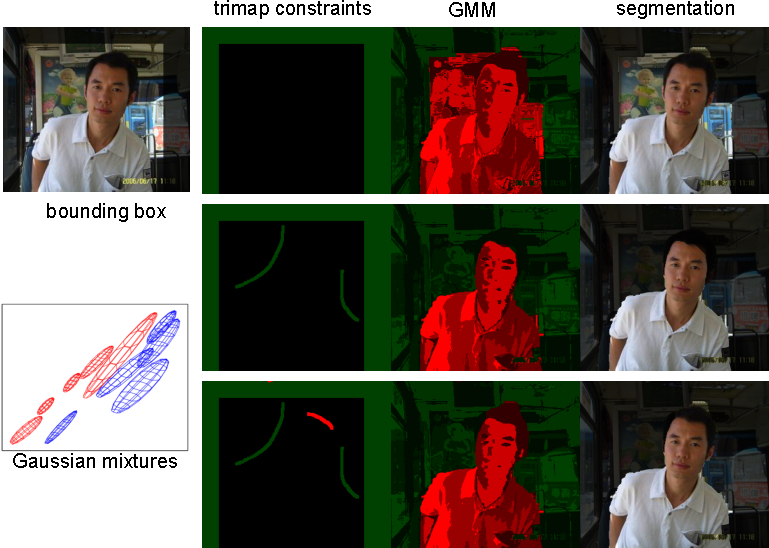
\includegraphics[width=1\textwidth]{figures/grabcut/gc}
\end{frame}

\begin{frame}
  \frametitle{Prior}
  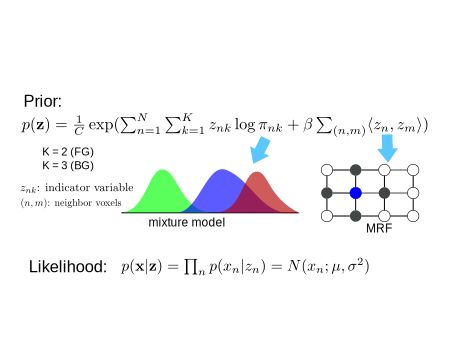
\includegraphics[width=1\textwidth]{figures/prior}
\end{frame}

\begin{frame}
  \frametitle{Prediction Score}
  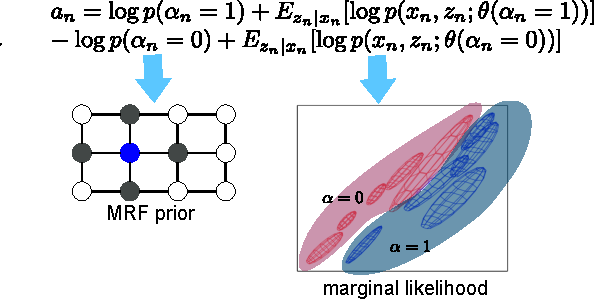
\includegraphics[width=1\textwidth]{figures/logistic}
\end{frame}
\end{document}
